\section{Validation and Verification}
\todo{Move parts to Evaluation}
In this section, we first describe how the system is tested and how we verify the quality of the code with SIG \cite{sig}. Afterwards we define a protocol with which the results of the system can be evaluated for correctness. We will first evaluate the results of the classification, and then the relation scores. These are related in the sense that a relation score is calculated by the number of occurrences in labelled documents, so the correctness of labelling affects the correctness of relation scores.\\

\subsection{Testing the Application}
We will test the program using four different testing methods. As framework we will use pytest\cite{pytest} which is integrated in python. The first is unit testing, which tests the separate components individually. Next comes integration testing, to see how well different components work together. Afterwards we use system testing for testing the different system components. Lastly, acceptance testing is used for testing how well the clients think the program works.

\subsubsection{Unit Testing}
Unit testing is done by writing automatic tests and making sure they pass every time the tests are executed. Unit tests test each method of a function separately, checking that the method does what it is supposed to do. If the method would need information from outside the class that information is mocked. This means that instead of using that other class, a fake object is made which returns a fake value. This ensures the tests will never fail due to changes in other classes. We achieved a test coverage of 85\%.

\subsubsection{Integration Testing}
Integration testing uses automated tests which test how well different components of the system work together. This is done more or less the same as unit testing, however whilst you would mock methods from other classes in unit testing, with integration testing you do not. It is assumed that the separate modules are unit tested, therefor if an error occurs it is because something is wrong with the interaction between the modules and not with the modules themselves. 

\subsubsection{System Testing}
We also used system testing. System testing provides a more complete test of the entire system. This means it is useful to detect faults in the overall system, but less easy to determine where these faults may be located. System testing is done manually, which means the tests can not be easily repeated when the system changes whilst with other testing techniques this is possible.

\subsubsection{Acceptance Testing}
Last we used acceptance testing. This is testing done to see if the software does what the clients are expecting it to do. These tests are therefore also executed by the clients manually. Afterwards they can say what worked, what did not work, what was missing and what could be improved. For this, we set up an evaluation protocol.\\

\subsection{SIG}
SIG \cite{sig}, short for software improvement development group, is an organisation that analyses the code of projects to give insights in the quality of how the code is written. A high score means the code is highly maintainable and is kept simple. SIG includes Better Code Hub \cite{better_code_hub} which checks our code according to 10 guidelines as can be seen in appendix \ref{A_better_code_hub_guidelines}. The great thing about Better Code Hub is that it can be run at anytime. We can check Better Code Hub whenever, whilst for SIG we have to send in our code and wait for feedback. 

\subsubsection{week 5}
The first feedback from SIG was in the fifth week of development. Before uploading on BetterCodeHub our code passed all checks. For SIG it had a score from four out of five stars which means our code is above average maintainable. The last star was missed because the code is above average complex. This means that some of the functionality of some methods should be split into separate methods.

\subsubsection{week 9}
Since the upload date for SIG is the same date as the due date of the final report we can not present the second SIG review. Instead we will present the results from BetterCodeHub, run on the last day before the due date of the report. This time there were two issues which resulted in a score of 8/10. The first was with keeping unit interfaces small, which resulted from a method with too many parameters. However since the different parameters are not part of a same object we did not take time better spent elsewhere to refactor this. The other issue was with coupling architecture components loosely, which resulted from our workers being used for different parts of the application.

\subsection{Evaluating the Classification}
There are several ways to evaluate machine learning algorithms. We will base our evaluation of the classifier on the guidelines of the Microsoft Azure Machine Learning evaluation model \cite{EvualteML}. According to the page binary classification can be evaluated with the following metrics: Accuracy, Precision, Recall, F1 and AUC. Note that we will use a one vs the rest strategy, meaning all classes will be separately evaluated.

\subsubsection{Accuracy}
Accuracy is the proportion of correctly classified instances. This however a poor indication of how well the classifier works. For instance if you have a test set of 100 websites, of which 90\% belongs to Category A. Than if the classifier simply predicts all websites to belong to category A the accuracy would be 90\%. It would seem the classifier performs well, but it actually fails to classify the other 10\% of the websites correctly.

\subsubsection{Confusion Matrix}
A page can only either belong to class A (positive), or not belong to class A (negative). If a page is predicted by the classifier correctly it is called true positive (TP) or true negative (TN). If the classifier predicts the page incorrectly it results in a false positive (FP) or false negative (FN). This can be seen in the confusion matrix in figure \ref{fig:confusion_matrix}. 

\begin{figure}[ht]
\centering
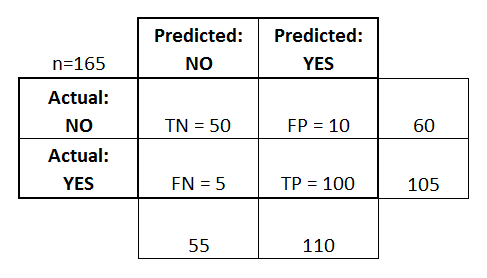
\includegraphics[width=0.5\textwidth]{confusion_matrix}
\caption{confusion matrix \protect\footnotemark{}}
\label{fig:confusion_matrix}
\end{figure}
\footnotetext{\url{https://docs.microsoft.com/en-us/azure/machine-learning/machine-learning-evaluate-model-performance}}


\subsubsection{Precision, Recall, F1 and UAC}
The \textbf{precision} of the classifier is the proportion of positives that are classified correctly: $\frac{TP}{TP+FP}$. This is used for questions such as "Out of the pages that were classified as category A, how many were classified correctly?".\\

the \textbf{recall} of the classifier is used to answer the question "What percentage of the pages that fit category A were classified correctly?". In other words: $\frac{TP}{TP+FN}$.

The \textbf{F1 Score} uses both precision and consideration. It is computed by using the following formula: $F1 = 2\cdot \frac{precision \cdot recall}{precision + recall}$. The F1 score summarised evaluation in a single number, but for evaluation it is better to use recall and precision to understand the behaviour of the classifier. \\

The \textbf{Receiver Operating Characteristic (ROC) curve} and the corresponding \textbf{Area Under the Curve (AUC) value} can be used to inspect the true positive rate (Recall) vs. the false positive rate $\frac{FP}{FP + TN}$. To do this, the possibilities pages are correctly classified are needed. For each threshold on these probabilities for the classifier, the true positive rate and the false positive rate are calculated and are plotted in a graph, which results in something like \ref{fig:UAC}. The closer the ROC curve is to the upper left corner, the better the classifier's performance is. When close to the diagonal of the plot, the classifier tends to make predictions close to random guessing. The UAC value is the are under the ROC curve.

\begin{figure}[ht]
\centering
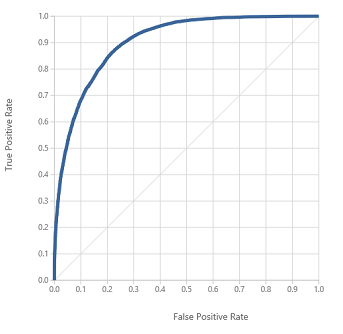
\includegraphics[width=0.5\textwidth]{UAC}
\caption{ROC / UAC graph \protect\footnotemark{}}
\label{fig:UAC}
\end{figure}
\footnotetext{\url{https://docs.microsoft.com/en-us/azure/machine-learning/machine-learning-evaluate-model-performance}}

\subsection{Evaluation of Relation Scores} \label{sec:validation_protocol}
Evaluating relation scores is done differently. An important factor here is that cities have a natural relation due to their geographical position \cite{tobler1970computer}, so one would expect cities that lie close to each other are more related than cities that are on different sides of the country. This natural relation can be represented using the Gravity Model by Reilly \cite{reilly1931law}. The Gravity Model describes that the expected relation between two cities is based on the population of the two cities and the distance between these cities. A relation between two cities that is extracted from the data should thus expose a similar relative score as they would for the gravity model. Consider for example Amsterdam and Hoofddorp, which are cities that lie close to each other. Amsterdam is a large city, whereas Hoofddorp is much smaller. However, due to their close geographical position, the score that results from the Gravity Model would be high. If they turn out to have a very high score in our system, that would imply that the system is correct. Besides the Gravity Model, one can rely on the opinion of an expert in the field of urbanism that can judge whether an extracted relation is close to reality or not. We therefore agreed with the client that they would decide on a small set of relations whether they are correct. Lastly, the relations in the Randstad, a large urban area with the four largest cities of the Netherlands, have been examined before on the basis of firms \cite{van2010economic}. These relations can be compared to those extracted by the system.